%%%%%%%%%%%%%%%%%%%%%%%%%%%%%%%%%%%%%%%%%%%%%%%%%%%%%%%%%%%%%%%%%%%%%%%%%%%%%%%%%%%%%%%%
%%
%%  Última alteração em 08/2013 por Rafael Pasquini (WTDCC 2013)
%%
%%%%%%%%%%%%%%%%%%%%%%%%%%%%%%%%%%%%%%%%%%%%%%%%%%%%%%%%%%%%%%%%%%%%%%%%%%%%%%%%%%%%%%%%

\documentclass[11pt]{article}
\usepackage{sbc-template}
\usepackage{graphicx,url}
%\usepackage[dvips]{graphicx}
%\usepackage[pdftex]{color,graphicx}
\usepackage{multicol}
\usepackage{multirow}
\usepackage{verbatim}
\usepackage{array}
\usepackage{amssymb,amsmath}
\usepackage[brazilian]{babel}
\usepackage[utf8]{inputenc}
\usepackage[T1]{fontenc}
\usepackage{tabularx}

\sloppy

\title{2$^o$ Trabalho de Inteligência Computacional - Data Mining}

\author{Autor: Gustavo Rezende Silva,\\ Orientador:Gina Maira Barbosa
de Oliveira}


\address{Faculdade de Computação\\
 Universidade Federal do Uberlândia (UFU)\\
  Uberlândia -- MG -- Brasil
  \email{gustavorezendesilva@hotmail.com, gina@ufu.br}
}

\begin{document}

\maketitle


\begin{resumo}
Este trabalho tem como intuito desenvolver um algoritmo genético para realizar
uma mineração de dados em uma base dermatológica, de maneira a gerar regras de
classificação para as diversas classes da doença erythemato-squamous presentes
neste banco de dados.
\end{resumo}

\begin{palavraschave}
algoritmos genéticos, data mining, mineração de dados, inteligência computacional
\end{palavraschave}

\section{Introdução}
\label{sec:intro}

Atualmente a quantidade de banco de dados armazenados por supermecados, hospitais,
empresas de marketing e muitos outros tipos de empresas vem aumentado significativamente.
Com isso, técnicas para extrair e analisar informações de grandes bases têm sido
desenvolvidas e este conjunto de ferramentas e técnicas é definida como
mineração de dados (data mining).

Na área médica existe um grande interesse em desenvolver ferramentas para extrair
informações de bancos de dados de pacientes com o intuito de auxiliar os médicos
a diagnosticar os mesmos, devido ao grande potêncial do data mining este vem sido
 utilizado. Neste trabalho aplicou-se algumas técnicas de mineração
de dados para extrair informações de um banco de dados dermatológico disponível
no repositório \textit{Machine Learning repository} da UCI.

Esta base contém informações sobre pacientes diagnosticados com alguma das
variações da doença chamada \textit{erythemato-squamous}. O diagnóstico dos
diferentes tipos desta enfermidade é complicada, pois a variação entre elas
é pequena.

O objetivo final da análise deste banco de dados é conseguir extrair uma regra
para cada uma das variações da doença \textit{erythemato-squamous} presentes na
base. De formar que um paciente informando apenas os seus sintomas possa ser classificado
com alguma das enfermidades, e este resultado pode ser utilizado pelo médico
como referência para o diagnóstico.

\section{Desenvolvimento}
\label{sec:desen}

Com o intuito de gerar regras para a base dermatológica citada na sec.
\ref{sec:intro} foi desenvolvido um algoritmo genético seguindo o artigo de
Fidelis \textit{et al.}(2000) e Miranda \textit{et al.}(2003). Nestes trabalhos o indivíduo é uma
abstração da regra de classificação de uma classe específica da doença
\textit{erythemato-squamous}, ou seja, o que define se um paciente é
pré-diagnosticado com uma das enfermidades classificadas.

No banco de dados utilizado cada paciente é representado por um número e 34
atributos que representam os sintomas das doenças, por isso um indivíduo é
composto por 34 atributos, 34 operadores matemáticos($=$, $!=$, $<$ ou $>=$) e
34 pesos (fig. \ref{fig:individuo}). De forma que um atributo relacionado com um
operador define uma condição para um paciente ser classficado naquela regra
(Ex.: atributo 2 >= 1), e ainda o peso é um número real entre 0 e 1 que
representa a probabilidade de uma condição aparecer na regra.

\begin{figure}
  \centering
  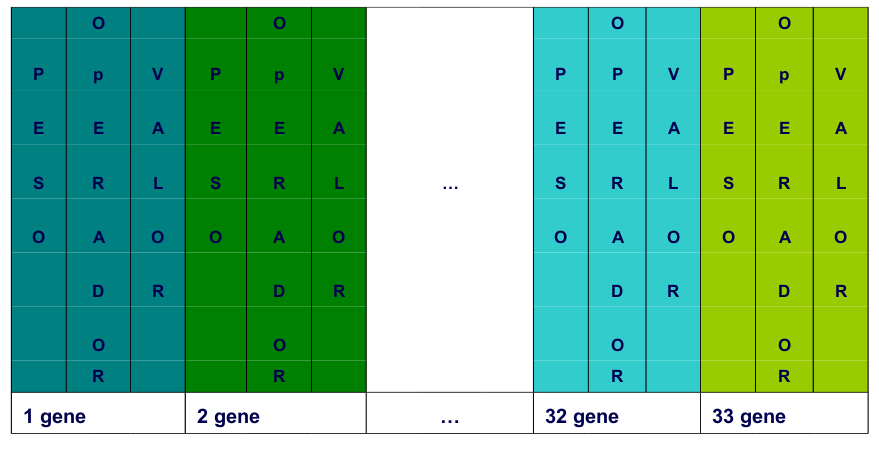
\includegraphics[width=8cm]{individuo.png}
  \caption{Representação de um indivíduo}
  \label{fig:individuo}
\end{figure}

Como parâmetros do algoritmo genético adotou-se uma população inicial de
50 individuos, taxa de cross over de 100\%, taxa de mutação de 30\%, número de
gerações igual a 50. A atualização da população é feita ordenando os pais e
filhos em ordem crescente de avaliação e pegando os 50 melhores, e configurou-se
como valor máximo de peso para o qual uma condição aparece sendo 0,3.

Para treinar o algoritmo e gerar as regras foi utilizado $2/3$ da base, em seguida
após as regras serem geradas as mesmas foram testadas utilizando o $1/3$ restante
dos dados.

Outro aspecto importante é o método de avaliação adotado, neste trabalho
para atribuir uma nota ao indivíduo foi utilizada a equação \ref{eq:av}.

\begin{equation} \label{eq:se}
  S_e = \frac{T_p}{T_p +F_n}
\end{equation}

\begin{equation} \label{eq:sp}
  S_e = \frac{T_n}{T_n +F_p}
\end{equation}

\begin{equation} \label{eq:av}
  Av = S_e * S_p
\end{equation}

Onde:\newline
\begin{itemize}
    \item $T_p$ - Verdadeiros positivos\newline
    \item $T_n$ - Verdadeiros negativos\newline
    \item $F_p$ - Falsos positivos\newline
    \item $F_n$ - Falsos negativos\newline

\end{itemize}

\section{Análise dos Resultados}
\label{sec:resultados}

O algoritmo genético desenvolvido para mineração de dados foi executado 10 vezes
para cada classe da doença, em seguida o melhor resultado de cada classe foi
escolhido e estes estão representados na tabela \ref{tab:etapa1}.

\begin{table}[h]
  \centering
  \begin{tabular}{|c|l|c|c|}
    \hline
    Classe & \multicolumn{1}{c|}{Regras}  & Fitness & Fitness\\
    das Doenças &  & Treinamento & Teste\\
    \hline
    \multirow{2}{*}{1} & thinning of the suprapapillary epidermis >= 1 & 0.929820 & 0.996290 \\
    & focal hypergranulosis < 3 & &\\
    \hline
    \multirow{6}{*}{2} & follicular papules  = 0 & 0.829799 & 0.765162\\
    & fibrosis of the papillary dermis < 1 & &\\
    & exocytosis != 0 & &\\
    & clubbing of the rete ridges < 1 & &\\
    & vacuolisation and damage of basal layer != 3 & &\\
    & band-like infiltrate < 1 & &\\
    \hline
    \multirow{2}{*}{3} & elongation of the rete ridges = 0 & 0.992163 &0.994803\\
    & band-like infiltrate >= 2 & &\\
    \hline
    \multirow{5}{*}{4} & family history != 1 & 0.811603 & 0.814022 \\
    & eosinophils in the infiltrate < 1 & &\\
    & elongation of the rete ridges == 0 & &\\
    & saw-tooth appearance of retes < 2 & &\\
    & follicular horn plug != 2 & &\\
    \hline
    \multirow{6}{*}{5} & koebner phenomenon  == 0 & 0.996662 & 0.991431 \\
    & oral mucosal involvement  != 1 & &\\
    & knee and elbow involvement  < 3 & &\\
    & PNL infiltrate != 2 & &\\
    & fibrosis of the papillary dermis != 0 & &\\
    & band-like infiltrate != 3 & &\\
    \hline
    \multirow{2}{*}{6} & follicular papules  >= 1 & 0.991299 & 0.986765 \\
    & perifollicular parakeratosis != 0 & &\\
    \hline
  \end{tabular}
  \caption{Resultados do data mining}
  \label{tab:etapa1}
\end{table}

Para escolher o melhor resultado foi levado em consideração a avaliação de
treinamento e teste, além do número de condições resultantes. Uma vez que uma
regra com muitas condições não representa o problema de forma genérica, apenas
aquele conjunto de dados específicos.

Com a intenção de se ter uma ideia geral do resultado das regras obtidas, as médias
dos melhores resultados de cada execução para a mesma regra foram calculadas e
se encontram na tabela \ref{tab:medias}.

\begin{table}[h]
  \centering
  \begin{tabular}{|c|c|c|}
    \hline
    \multirow{2}{*}{Classe} & Média Fitness & Média Fitness \\
    & Treinamento & Teste \\
    \hline
    1 & 0.932275 & 0.981523\\
    \hline
    2 & 0.825245 & 0.850473\\
    \hline
    3 & 0.976214 & 0.969933\\
    \hline
    4 & 0.850391 & 0.725871\\
    \hline
    5 & 0.896647 & 0.831133\\
    \hline
    6 & 0.939587 & 0.809525\\
    \hline
  \end{tabular}
  \caption{Média das avaliações de cada classe}
  \label{tab:medias}
\end{table}

Ao comparar os resultados obtidos neste trabalho com os de Fidelis \textit{et al.}(2000) e
Miranda \textit{et al.}(2003), percebe-se que as avaliações das regras encontradas
são bem próximas. Entretanto, as condições associadas a cada regra variam em quase
todas elas.

Em seguida, alguns parâmetros do algoritmo genético foram alterados com o intuito
de obter melhores resultados.

Alterando apenas o peso máximo permito o resultados encontrados foram diferentes
(tabela \ref{tab:etapa2-1}).
Para algumas classes como a 1 e 2 as avaliações foram melhores, já na classe 5
o fitness foi igual porém a quantidade de condições foi menor, a classe 3 permaneceu
com as mesmas avaliações e a 4 e 6 pioraram.

\begin{table}[h]
  \centering
  \begin{tabular}{|c|l|c|c|}
    \hline
    Classe & \multicolumn{1}{c|}{Regras}  & Fitness & Fitness\\
    das Doenças &  & Treinamento & Teste\\
    \hline
    \multirow{2}{*}{1} & clubbing of the rete ridges >= 1 & 0.955212 & 0.996290 \\
    & perifollicular parakeratosis < 1  & &\\
    \hline
    \multirow{6}{*}{2} & koebner phenomenon  < 1 & 0.910755 &  0.923471 \\
    & polygonal papules  == 0 & &\\
    & fibrosis of the papillary dermis < 1 & &\\
    & elongation of the rete ridges != 3 & &\\
    & thinning of the suprapapillary epidermis == 0 & &\\
    & perifollicular parakeratosis == 0 & &\\
    \hline
    \multirow{2}{*}{3} & PNL infiltrate == 0  & 0.992163 &0.994803\\
    & band-like infiltrate >= 2 & &\\
    \hline
    \multirow{5}{*}{4} & koebner phenomenon  >= 1 & 0.892055 &  0.727187  \\
    & scalp involvement != 2 & &\\
    & melanin incontinence < 1 & &\\
    & exocytosis >= 1  & &\\
    & clubbing of the rete ridges < 1  & &\\
    & thinning of the suprapapillary epidermis != 2   & &\\
    \hline
    \multirow{6}{*}{5} & polygonal papules  < 2  & 0.996662 & 0.991431 \\
    & fibrosis of the papillary dermis != 0  & &\\
    &  hyperkeratosis < 3  & &\\
    & focal hypergranulosis < 1 & &\\
    \hline
    \multirow{2}{*}{6} & koebner phenomenon  != 2  & 0.986932 & 0.986765 \\
    & perifollicular parakeratosis >= 1 & &\\
    \hline
  \end{tabular}
  \caption{Peso máximo = 0.2}
  \label{tab:etapa2-1}
\end{table}

As maiores dificuldades na reprodução dos modelos foi conseguir analisar os
resultados e compara-los, e ainda entender que um número grande de condições
não satisfaz o propósito da mineração de dados.

\nocite{*}
\bibliographystyle{sbc}
\bibliography{bib}

\end{document}
